\chapter{Compatibiliteit van herkenningssystemen}
Voor het herkenningssysteem bestuderen we de implementatie van de ResNet50 architectuur die in paragraaf \ref{resnet} werd besproken.
We vertrekken hierbij met een bestaand model dat voorgetraind is met het TensorFlow of het PyTorch framework.
Om vervolgens de mogelijke paden te bestuderen naar een mobiele implementatie.
Hierbij zullen we gebruik maken van Google Colaberate ... om de modellen in te laden en te converteren.
Om het geconverteerd model te implementeren op een mobiel toestel zullen we gebruik maken van Android Studio ....

% \section{ResNet50}
% \cite{he2015deep} heeft vastgesteld dat als het aantal lagen van een CNN toeneemt dat op een bepaald moment de training accuraatheid daalt.
% Dit verschijnsel noemt men de vanishing gradient.
% In paragraaf \ref{train} hebben we besproken hoe we de gradient kunnen berekenden tijdens het trainen van een CNN.
% Voor elke laag in het CNN moet de gradient opnieuw berekend worden door telkens opnieuw de afgeleide te berekenen.
% Hierdoor wordt de gradient steeds kleiner en kleiner tot deze een minimum bereikt.
% Waardoor de gewichten in de eerste lagen heel traag aanpassen of zelfs niet meer veranderen.
% \cite{he2015deep} die dit probleem hebben vastgesteld hebben dit opgelost door gebruik te maken van skip connections.
% Hierbij wordt de input van een laag rechtstreeks met een volgende laag die x aantal lagen verder ligt.
% Op deze manier worden de gradienten per laag niet meer kleiner.
% ResNet50 bestaat uit 50 convolutie lagen waarbij er een skip connection plaatsvindt per 3 lagen.
% De resnet50 architectuur is opgebouwd uit ResNet blokken die bestaan uit 3 convolutie lagen en 1 skip connection.

%https://github.com/tensorflow/models/blob/master/official/vision/image_classification/resnet/resnet_model.py
%https://github.com/priya-dwivedi/Deep-Learning/blob/master/resnet_keras/Residual_Networks_yourself.ipynb

\section{Van TensorFlow naar mobiel framework}
Voor het experiment van ResNet50 maken we gebruik van het standaard ResNet50 netwerk dat in TensorFlow ge\"implenteerd kan worden vanuit Keras.
Dit ResNet50 model is voorgetrained op de ImageNet dataset ... 
Dit netwerk kan vervolgens hertrained voor een gewenste functionaliteit.
Voor deze implementatie zullen we echter vertrekken van het ResNet50 Keras model dat reeds bestaat.

\subsection{TensorFlow Lite implementatie} \label{tf_h_conv}
Het inladen en converteren van het Keras model kan eenvoudig via de volgende lijnen code.

\begin{python}
model = tf.keras.applications.resnet50.ResNet50() # model inladen
converter = tf.lite.TFLiteConverter.from_keras_model(model) # init converter
tflite_model = converter.convert() # model converteren
open('model.tflite', 'wb').write(tflite_model) # model opslaan
\end{python}

Het ResNet50 model kan zonder problemen of aanpassingen rechtstreeks worden geconverteerd naar TFlite.
In tabel \ref{tab:TFop} is te zien welke operaties er zijn terug te vinden in het TensorFlow ResNet50 model dat is ingeladen.
Vervolgens is in de tabel ook terug te vinden wat er met de operaties gebeurt tijden de TFLite conversie.
In de tabel kunnen we zien welke TensorFlow operaties worden ondersteund door een TFLite equivalent.
Vervolgens kunnen we in de tabel ook zien op welke operaties optimalisaties worden uitgevoerd tijdens het converteren.
Bij deze optimalisaties worden operaties samengevoegd, verwijderd of vervangen door een constante.
In figuur \ref{fig:class_opt} kunnen we zien welke optimalisaties er worden uitgevoerd op een ResNet50 convolutieblok.

\begin{figure}[!ht]
	\centering
	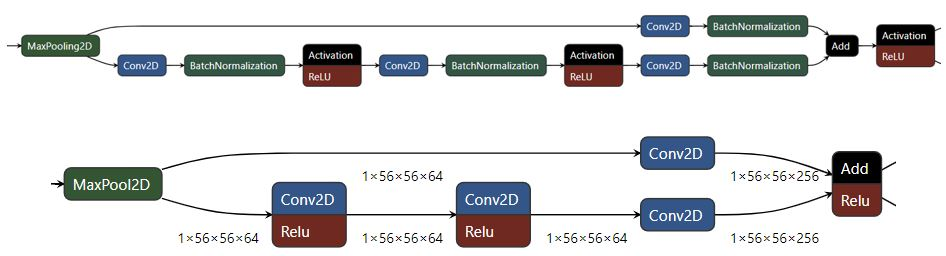
\includegraphics[width=1.0\linewidth]{fig/class_opt.jpg}
	\caption{ResNet50 convolutieblok voor en na TFLite conversie. BatchNorm en ReLu zijn hierbij samengevoegd met de Conv2D opperaties.}
	\label{fig:class_opt}
\end{figure}

Voor de android implementatie kunnen we metadata aan het model toevoegen.
\begin{python} 
ImageClassifierWriter = image_classifier.MetadataWriter
model_p = "./model.tflite" # TFLite model
label_p = "./labels.txt" # label file voor label formaat
save_p = "./model_meta.tflite" # opslaan pad
input_norm_mean = 0.0
input_norm_std = 1.0
    
# metadata scrijver
writer = ImageClassifierWriter.create_for_inference(
    writer_utils.load_file(model_p), [input_norm_mean], [input_norm_std],
    [label_p])
    
# Voeg metadata aan het model toe en sla op
writer_utils.save_file(writer.populate(), save_p)
\end{python}

Doordat we deze metadata hebben toegevoegd heeft android studio toegang tot al de relevante input en output informatie.
Vermits Android studio toegang heeft tot deze informatie kan het zelf code genereren om het TFLite model te implementeren.
De code die gegenereerd wordt is implementeerbaar in Java en Kotlin.

\subsection{ONNX implementatie} \label{classonnx}
Het TensorFlow model kunnen we converteren naar ONNX met Tf2onnx bibliotheek.
De tf2onnx bibliotheek ondersteund TensorFlow en TFLite, dus we kunnen bijde modellen converteren.
In tabel \ref{tab:TFop} is te zien welke operaties operaties ondersteund zijn door ONNX.
Ook is te zien vanaf welke opset versie deze operaties worden ondersteund.
Hierbij kunnen we zien dat de minimale opset versie 6 moet zijn vanwege de FusedBatchNormV3 operatie die pas vanaf versie 6 wordt ondersteund.
Via de volgende lijn code kunne we het TensorFlow model converteren naar ONNX.
Of we kunnen het TFLite model converteren naar ONNX door de optie --tflite mee te geven.

\begin{python}
python -m tf2onnx.convert --saved-model ./model --output model.onnx
\end{python}

Voor de android implementatie van het ONNX model maken we gebruik van Kotlin in plaats van Java.
De voornaamste reden hiervoor is dat de Onnxruntime documentatie Kotlin code gebruikt voor de Java API.
%voorbeelden ook in Kotlin zijn ge\"implementeerd.
Via onderstaande code kan het ONNX model worden uitgevoerd in Android studio.

\begin{python} 
var env = OrtEnvironment.getEnvironment()
// lees het ONNX model als byteArray
var session = env.createSession(resources.openRawResource(R.raw.model_tf).readBytes())
// Maak een input tensor aan
var input_tensor = OnnxTensor.createTensor(env, imgData, shape)
// maak een inputmap aan
var inputs = Collections.singletonMap("input_1", t1)
// voer model uit
val output = session?.run(inputs)
\end{python}

We lezen het ONNX model in als een byteArray.
Dit ONNX model is opgelsagen in de res/raw folder van het Android studio project.
Vervolgens wordt er een ONNX input tensor aangemaakt.
Hierbij wordt de afbeelding data als FloatArray meegegeven en de vorm van de input tensor die het ONNX model verwacht.
Het ONNX model verwacht een input vorm [1, hoogte, breedte, 3] deze vorm is van het NCHW formaat \ref{nhwc}.
Voordat we het model kunnen uitvoeren moeten we de input tensor aan een map toevoegen.
De keys van deze map zijn de input namen van het ONNX model, de values van de map zijn de input tensoren.
De input namen zijn terug te vinden in de output boodschapen van tf2onnx converter.
%We moeten er wel bij vermelden dat TFLite enkel variabelen van het type float32 en int8 ondersteund.
%De tf2onnx converter maakt standaard gebruik van ONNX opset versie 9.
%Bij het converterent van TensorFlow naar ONNX onder standaard omstandigheden krijgen we de volgende fout 
%\textcolor{red}{ValueError: StridedSlice: only strides=1 is supported}.  
%Voor het converteren van TensorFlow naar ONNX is minstens opset versie 10 nodig.

\begin{table}[!ht]
    \caption{Alle operaties die terug te vinden zijn in het ResNet50 model en hun compatibiliteit met andere frameworks}
\begin{tabular}{ccc}
    \hline
    TensorFlow Operaties & TensorFlow \textrightarrow TFLite & ONNX Opset \\
    \hline
    AddV2 & Ondersteund & 1 \\
    BiasAdd & Samengevoegd & 1 \\
    %Const & constant & 1 \\
    Conv2D & Ondersteund & 1 \\
    FusedBatchNormV3 & Samengevoegd & 6 \\
    Identity & Verwijderd & 1 \\
    MatMul & Ondersteund & 1 \\
    MaxPool & Ondersteund & 1 \\
    Mean & Ondersteund & 1 \\
    NoOp & Verwijderd & / \\
    %Pack & Ondersteund & 1 \\
    Pad & Ondersteund & 1 \\
    Placeholder & Constant & 1 \\
    Relu & Samengevoegd & 1 \\
    Softmax & Ondersteund & ? \\
    StatefulPartitionedCall & Ondersteund & / \\
    \hline
\end{tabular}
\label{tab:TFop}
\end{table}

\section{Van PyTorch naar mobiele implementatie}
Voor de PyTorch implementatie maken we gebruik van het ResNet50 model uit de Torchvision bibliotheek.
Dit model is voorgetraind op de ImageNet dataset ... .
Dit netwerk kan vervolgens hertrained voor een gewenste functionaliteit.
Voor deze implementatie zullen we echter vertrekken van het ResNet50 Keras model dat reeds bestaat.

\subsection{PyTorch Mobile implementatie} \label{py_class}
Via de volgende lijnen code kunnen we een ResNet50 Torchvision model inladen en converteren voor mobiel gebruik.

\begin{python}
model = models.resnet50(pretrained=True) # model inladen
model.eval() # model in uitvoer modus
example = torch.rand(1, 3, 224, 224) # voorbeeld input
# Torchscript module genereren
traced_script_module = torch.jit.trace(model, example) 
# optimalisaties voor mobiel gebruik uitvoeren op de scriptmodule
traced_script_module_optimized = optimize_for_mobile(traced_script_module)
# model opslaan voor mobiel gebruik
traced_script_module_optimized._save_for_lite_interpreter("./model.pt") 
\end{python}

Het ResNet50 model wordt zonder problemen geconverteerd, geoptimaliseerd en opgeslagen voor mobiel gebruik.
De 
\begin{table}[!ht]
    \caption{Alle operaties die terug te vinden zijn in het ResNet50 model en hun compatibiliteit met andere frameworks}
\begin{tabular}{ccc}
    \hline
    TorchScript & TorchScript \textrightarrow  ge\"optimaliseerd torchscript & ONNX Opset \\
    \hline
    Add & Ondersteund & 1 \\
    AdaptiveAvgPool2d & Ondersteund & 1 \\
    BatchNorm2d & Samengevoegd & 1 \\
    Conv2d & Ondersteund & 1 \\
    Flatten & Ondersteund & 1 \\
    Linear & Ondersteund & 1 \\
    MaxPool2d & Ondersteund & 1 \\
    ReLu & Samengevoegd & 1 \\
    \hline
\end{tabular}
\label{tab:PYop}
\end{table}
\section{Conclusie}

Het model kan vervolgens eenvoudig ge\"implementeerd worden in android studio.
\begin{python}
module = Module.load(assetFilePath(MainActivity.this, "model.ptl"));
Tensor inputTensor = TensorImageUtils.bitmapToFloat32Tensor(bitmap,
            TensorImageUtils.TORCHVISION_NORM_MEAN_RGB, 
            TensorImageUtils.TORCHVISION_NORM_STD_RGB);
Tensor outputTensor = module.forward(IValue.from(inputTensor)).toTensor();
\end{python}

\subsection{ONNX implementatie}
Het ResNet50 Torchvision model is eenvoudig te converteren naar ONNX via de volgende lijnen code.
\begin{python}
torch.onnx.export(model, # model 
    example,             # model input
    "model_py.onnx",     # waar opslaan
    export_params=True,        # slaag parameters op in model file
    input_names = ['input_1'], # input namen
    output_names = ['output']) # output namen    
\end{python}

Het gegenereerde ONNX model kan ge\"implementeerd worden in android studio.
Het ONNX model verwacht een input vorm [1, 3, hoogte, breedte] deze vorm is van het NCHW formaat \ref{nhwc}.
Ook verwacht het geconverteerd pytorch model een genormaliseerde input afbeelding.
De genormaliseerde waarde kan via de volgende formule berekent worden.
\newline
\newline
$genormaliseerd = (waarde - mean) / std $
\newline
$mean = \{0.485, 0.456, 0.406\}$
\newline
$std = \{0.229, 0.224, 0.225\}$
\newline
\newline
Waarbij mean de gemiddelde waarde is en std de standaarddeviatie is waarmee Torchvision een normalisatie uitvoert.
De mean en std bevatten 3 waarde.
Dit is omdat bij Torchvision elk kleurkanaal zijn eigen mean en std waarde heeft voor normalisatie.
De rest van de implementatie in Android studio is identiek aan de ONNX implementatie van het TensorFlow model \ref{classonnx}. 

\section{ResNet50 resultaten}

\begin{table}[!ht]
    \caption{Binaire grootte van al de ResNet50 modellen}
\begin{tabular}{cccc}
    \hline
    Framework & Standaard model & Mobiel model & ONNX model \\
    \hline
    TensorFlow & 98.3MB & 97.45MB & 97.44MB \\
    PyTorch & 97.81MB & 97.44MB & 97.4MB \\
    \hline
\end{tabular}
\label{tab:class_size}
\end{table}

\begin{table}[!ht]
    \caption{Uitvoer snelheid van de modellen in Google Colab en voor de mobiele toepassingen gebruiken we de Xiaomi T9.}
\begin{tabular}{cccccc}
    \hline
    Framework & Standaard model & Mobiel model Colab & Mobiel model T9 & ONNX Colab & ONNX T9\\
    \hline
    TensorFlow & 0.209s & 0.366s & 1s & 0.115s & 1s \\
    PyTorch & 0.130s & 0.153s & 1s & 0.139s & 1s \\
    \hline
\end{tabular}
\label{tab:class_speed}
\end{table}

\begin{table}[!ht]
    \caption{Top 1 accuraatheid van de standaard en modellen voor mobiel gebruik. De modellen zijn uitgevoerd op Google Colab en Xiaomi T9.}
\begin{tabular}{cccccc}
    \hline
    Framework & Standaard model & Mobiel model Colab & Mobiel model T9 & ONNX Colab & ONNX T9\\
    \hline
    TensorFlow & 0.209s & 0.366s & 1s & 0.115s & 1s \\
    PyTorch & 0.130s & 0.153s & 1s & 0.139s & 1s \\
    \hline
\end{tabular}
\label{tab:class_acc}
\end{table}